%!TEX root = tapp_whatif.tex
\section{Introduction}
\label{sec:introduction}
What-if analysis~\cite{hung17,deutch13} determines how a hypothetical update to a database instance affects the result of a query.
Consider the following what-if query: \textit{``How would a 10\% increase in sales  affect our company’s revenue this year?''}
While the result of this query can help an analyst to understand how revenue is affected by sales,
its practical utility is limited because it does not provide any insights about how this increase in sales could have been achieved in the first place.
We argue that this problem is not specific to this example, but rather is a fundamental issue with classical what-if analysis since the hypothetical update to the database is part of the input.
We propose \emph{historical what-if queries} (\emph{\abbrHW}), a novel type of what-if queries where the user postulates a hypothetical change to the transactional history of the database.





%


%

%

%
%
%

%

%


%
%
%
%
%
%
%
%
%
%
%
%
%
%
%
%
%
%
%

%%%%%%%%%%%%%%%%%%%%%%%%%%%%%%%%%%%%%%%%
\begin{figure}[t]
  \centering

    \resizebox{1\columnwidth}{!}{
      \begin{minipage}{1.5\columnwidth}
        \centering
        {\bf\large Order}\\[1mm]
    \begin{tabular}{|c|c|c|c|c|l}
      \thead{ID} & \thead{Customer} & \thead{Country} & \thead{Price} & \thead{ShippingFee} & \\ \cline{1-5}
       % $\cMarker{T_0}{6}{1}(\upMarker{I}{T_0}{2}{1}(x_1))$ &
                                                          11 & Susan  & UK &  20 &  5 & $o_1$ \\
    % $\cMarker{T_0}{6}{2}(\upMarker{I}{T_0}{3}{2}(x_2))$ &
      12 & Alex  & UK &  50 & 5 & $o_2$ \\
    % $\cMarker{T_0}{6}{4}(\upMarker{I}{T_0}{4}{3}(x_3))$ &
                                                          13 & Jack  & US &  60 & 3 & $o_3$ \\
       % $\cMarker{T_0}{6}{4}(\upMarker{I}{T_0}{5}{4}(x_4))$ &
                                                          14 & Mark  & US &  30 & 4 & $o_4$ \\ \cline{1-5}
    \end{tabular}
  \end{minipage}
} \vspace{-3mm}
  \caption{Running example database instance.}
  \label{fig:running-example-instance}
  \vspace{-4mm}
\end{figure}
%%%%%%%%%%%%%%%%%%%%%%%%%%%%%%%%%%%%%%%%
\begin{figure}[t]
  % \centering
  \resizebox{1\columnwidth}{!}{
    \begin{minipage}{1.5\linewidth}
      \centering
      \begin{tabular}{|l|l|c|}
        \hline
        \thead{U}                          & \multicolumn{1}{c|}{\thead{SQL}}                                                              \\ \hline
        \rowcolor{shadeblue}     $u_1$     & \lstinline! UPDATE Order SET ShippingFee=0  WHERE Price>=50;!                                \\  [1mm]
        \rowcolor{pink}         ${u_1}'$   & \lstinline! UPDATE Order SET ShippingFee=0  WHERE Price>=60;!                                \\ [1mm]
        $u_2$                              & \lstinline!  UPDATE Order SET ShippingFee=ShippingFee+5 WHERE Country='UK' AND Price <=100;!  \\[1mm]
        \rowcolor{shadeblue}        $u_3$  & \lstinline! UPDATE Order SET ShippingFee=ShippingFee-2 WHERE Price <=30 AND ShippingFee>=10;! \\ [1mm]
        \hline
      \end{tabular}
    \end{minipage}
  }                                                                                                                                       \\[-3mm]
  \caption{History $\history$ implementing the shipping fee policy and a hypothetical change of the policy (update ${u_1}'$ replaces $u_1$ to raise the price for waiving shipping fees to \$60).}
  \label{fig:Transitive-Transactions-Example}
\end{figure}
%%%%%%%%%%%%%%%%%%%%%%%%%%%%%%%%%%%%%%%%
%%%%%%%%%%%%%%%%%%%%%%%%%%%%%%%%%%%%%%%%
% \begin{figure}[t]
%   $,$                                                                                                                                                  \\[-7mm]
%   \centering
%   \resizebox{1\columnwidth}{!}{
%   \begin{minipage}{1.5\columnwidth}
%     \centering {\large \bf Order}                                                                                                                     \\[2mm]
%     \begin{tabular}{|c|c|c|c|c|c|c|l}
        %         \thead{ID} & \thead{Customer} & \thead{Item} & \thead{Quantity} & \thead{Price} & \thead{ShippingFee} & \thead{Status} &                       \\ \cline{1-7}
        %       %         $\cMarker{T_0}{6}{1}(\upMarker{I}{T_0}{2}{1}(x_1))$ &
                                                                                %                                                                                 11 & Susan  & X &  1 & 20 & 5 & Shipped & $o_1$                                            \\
                                                                                %    %                                                                                 $\cMarker{T_0}{6}{2}(\upMarker{I}{T_0}{3}{2}(x_2))$ &
                                                                                                                                                                                                                             %                                                                                                                                                                                                                              12 & Alex  & X &  2 & 20 & 5 & Received & $o_2$                                                                                                \\
                                                                                                                                                                                                                             %    %                                                                                                                                                                                                                              $\cMarker{T_0}{6}{4}(\upMarker{I}{T_0}{4}{3}(x_3))$ &
                                                                                                                                                                                                                                                                                                                                                                                                                                                                                                                       %                                                                                                                                                                                                                                                                                                                                                                                                                                                                                                                        13 & Jack  & Y &  2 & 30 & 3 & Received & $o_3$                                            \\
                                                                                                                                                                                                                                                                                                                                                                                                                                                                                                                       %       %                                                                                                                                                                                                                                                                                                                                                                                                                                                                                                                        $\cMarker{T_0}{6}{4}(\upMarker{I}{T_0}{5}{4}(x_4))$ &
                                                                                                                                                                                                                                                                                                                                                                                                                                                                                                                                                                                                                                                                                                                                                                                                                                                                                                                                                                                                                                                                                                              %                                                                                                                                                                                                                                                                                                                                                                                                                                                                                                                                                                                                                                                                                                                                                                                                                                                                                                                                                                                                                                                                                                               14 & Mark  & Z &  6 & 10 & 4 & Canceled & $o_4$                                            \\ \cline{1-7}
        %       \end{tabular}
        %         \end{minipage}
        %         }                                                                                                                                                    \\[-3mm]
        %         \caption{Database state after executing the original history}
        %         \label{fig:updated-example-instance}
        %%       \end{minipage}
        %         \end{figure}
        % %%%%%%%%%%%%%%%%%%%%%%%%%%%%%%%%%%%%%%%%
        %%%%%%%%%%%%%%%%%%%%%%%%%%%%%%%%%%%%%%%%
\begin{figure}[t]
  $\,$                                                                                                                                                   \\[-5mm]
  \centering
  \begin{minipage}{1\linewidth}
    \centering
    \resizebox{1\columnwidth}{!}{
      \begin{minipage}{1.5\columnwidth}
        \centering {\large \bf Order}                                                                                                                      \\[2mm]
        \begin{tabular}{|c|c|c|c|c|l}
          \thead{ID}                                                                                                                                                                                                                         & \thead{Customer} & \thead{Country} & \thead{Price} & \thead{ShippingFee} & \\ \cline{1-5}
          % $\cMarker{T_0}{6}{1}(\upMarker{I}{T_0}{2}{1}(x_1))$                                                                                                                                                                              &
                                                                  11                                                                                                                                                                         & Susan            & UK              & 20            & 8                   & $o_5$                                                        \\
                                                                  % $\cMarker{T_0}{6}{2}(\upMarker{I}{T_0}{3}{2}(x_2))$                                                                                                                      &
                                                                                                                          12                                                                                                                 & Alex             & UK              & 50            & 5                   & $o_6$ \\
                                                                                                                          % $\cMarker{T_0}{6}{4}(\upMarker{I}{T_0}{4}{3}(x_3))$                                                              &
                                                                                                                                                                                  13                                                         & Jack             & US              & 60            & 0                   & $o_7$                                                          \\
                                                                                                                                                                                  % $\cMarker{T_0}{6}{4}(\upMarker{I}{T_0}{5}{4}(x_4))$      &
                                                                                                                                                                                                                                          14 & Mark             & US              & 30            & 4                   & $o_8$                                                           \\ \cline{1-5}
        \end{tabular}
      \end{minipage}
    }                                                                                                                                                     \\[-3mm]
    \caption{Result of  executing the original history $\history$.}
    \label{fig:updated-example-instance}
  \end{minipage}
  % \begin{minipage}{0.27\linewidth}
  %   \centering
  %   \resizebox{1\columnwidth}{!}{
  %   \begin{minipage}{1.5\columnwidth}
  %     \centering {\large \bf Query result}                                                                                                                \\[2mm]
  %     \begin{tabular}{|c|c|l}
  %       \thead{Total} & \thead{Country}&                                                                                                                \\ \cline{1-2}
  %       73 & UK & $o'_1 + o''_2$                                                                                                                         \\
  %       94 & US & $o'_3 + o_4$                                                                                                                           \\
  %       \cline{1-2}
  %     \end{tabular}
  %   \end{minipage}
  % }                                                                                                                                                     \\[-3mm]
  %   \caption{$\query_{total}$ result}
  %   \label{fig:original-query-result}
  % \end{minipage}
\end{figure}
% %%%%%%%%%%%%%%%%%%%%%%%%%%%%%%%%%%%%%%%%
% %%%%%%%%%%%%%%%%%%%%%%%%%%%%%%%%%%%%%%%%
\begin{figure}[t]
  $\,$                                                                                                                                                   \\[-5mm]
  \centering
  \begin{minipage}{1\linewidth}
    \centering
    \resizebox{1\columnwidth}{!}{
      \begin{minipage}{1.5\columnwidth}
        \centering {\large \bf Order}                                                                                                                      \\[2mm]
        \begin{tabular}{|c|c|c|c|c|l}
          \thead{ID}                                                                                                                                                                                                                         & \thead{Customer} & \thead{Country} & \thead{Price} & \thead{ShippingFee}    & \\ \cline{1-5}
          % $\cMarker{T_0}{6}{1}(\upMarker{I}{T_0}{2}{1}(x_1))$                                                                                                                                                                              &
                                                                  11                                                                                                                                                                         & Susan            & UK              & 20            & 8                      & $o_5$ \\
                                                                  % $\cMarker{T_0}{6}{2}(\upMarker{I}{T_0}{3}{2}(x_2))$                                                                                                                      &
                                                                                                                          12                                                                                                                 & Alex             & UK              & 50            & \cellcolor{shadered}10 & $o_6'$ \\
                                                                                                                          % $\cMarker{T_0}{6}{4}(\upMarker{I}{T_0}{4}{3}(x_3))$                                                              &
                                                                                                                                                                                  13                                                         & Jack             & US              & 60            & 0                      & $o_7$                                                          \\
                                                                                                                                                                                  % $\cMarker{T_0}{6}{4}(\upMarker{I}{T_0}{5}{4}(x_4))$      &
                                                                                                                                                                                                                                          14 & Mark             & US              & 30            & 4                      & $o_8$                                                           \\ \cline{1-5}
        \end{tabular}
      \end{minipage}
    }                                                                                                                                                     \\[-3mm]
    \caption{Result of executing the hypothetical history $\ahmod$.}
    \label{fig:whatif-example-instance}
  \end{minipage}
  % \begin{minipage}{0.27\linewidth}
  %   \centering
  %   \resizebox{1\columnwidth}{!}{
  %     \begin{minipage}{1.5\columnwidth}
  %       \centering {\large \bf Query result}                                                                                                                \\[2mm]
  %       \begin{tabular}{|c|c|l}
  %         \thead{Total} & \thead{Country}                                                                                                                 \\ \cline{1-2}
  %         \cellcolor{shadered}78 & UK & $o'_1 + o'_2$                                                                                                     \\
  %         94 & US & $o'_3 + o_4$                                                                                                                           \\
  %         \cline{1-2}
  %       \end{tabular}
  %     \end{minipage}
  %   }                                                                                                                                                     \\[-3mm]
  %   \caption{$\query_{total}$ result}
  %   \label{fig:whatif-query-result}
  % \end{minipage}
\end{figure}
%%%%%%%%%%%%%%%%%%%%%%%%%%%%%%%%%%%%%%%%.

% %%%%%%%%%%%%%%%%%%%%%%%%%%%%%%%%%%%%%%%%
% \begin{figure*}[t]
%   \centering
%   \begin{minipage}{0.49\linewidth}
%   \centering
%     \resizebox{1\columnwidth}{!}{
%   \begin{minipage}{1.4\columnwidth}
%    \centering {\large \bf Employee}\\[2mm]
%     \begin{tabular}{l|c|c|c|c|c|l}
%      & \thead{ID} & \thead{Name} & \thead{Calls} & \thead{Sales} & \thead{Bonus} & \\ \cline{2-6}
%     $\cMarker{T_1}{22}{1}(\upMarker{U}{T_1}{21}{1}(\cMarker{T_0}{6}{1}(\upMarker{I}{T_0}{2}{1}(x_1)))$ & 101 & David Spears & 18 &  15 & 0 & $e'_1$ \\
% $\cMarker{T_0}{6}{2}(\upMarker{I}{T_0}{3}{2}(x_2))$ & 102 & Mark Smith & 40 &  20 & 100 & $e_2$ \\
%     $\cMarker{T_0}{6}{3}(\upMarker{I}{T_0}{4}{3}(x_3))$ &  103 & Susan Sommers & 80 &  50 & 200 & $e_3$ \\
%      $\cMarker{T_2}{24}{4}(\upMarker{U}{T_2}{23}{4}(\cMarker{T_0}{6}{4}(\upMarker{I}{T_0}{5}{4}(x_4)))$ &  104 & Robert Singer & 120 &  80 & 350 & $e'_4$ \\ \cline{2-6}
%     \end{tabular}
%   \end{minipage}
% }
%   \caption{Database state after executing the original history}
%   \label{fig:updated-example-instance}
% \end{minipage}
% % \end{figure}
% % %%%%%%%%%%%%%%%%%%%%%%%%%%%%%%%%%%%%%%%%
% % %%%%%%%%%%%%%%%%%%%%%%%%%%%%%%%%%%%%%%%%
% % \begin{figure}[t]
%   \begin{minipage}{0.49\linewidth}
%   \centering
% \resizebox{1\columnwidth}{!}{
%   \begin{minipage}{1.4\columnwidth}
%    \centering {\large \bf Employee}\\[2mm]
%     \begin{tabular}{l|c|c|c|c|c|l}
%       & \thead{ID} & \thead{Name} & \thead{Calls} & \thead{Sales} & \thead{Bonus} & \\ \cline{2-6}
%     $\cMarker{T_1}{22}{1}(\upMarker{U}{T_1}{21}{1}(\cMarker{T_0}{6}{1}(\upMarker{I}{T_0}{2}{1}(x_1)))$ & 101 & David Spears & 18 &  15 & 0 & $e'_1$ \\
% $\cMarker{T_3}{26}{2}(\upMarker{U}{T_3}{25}{2}(\cMarker{T_1}{22}{2}(\upMarker{U}{T_1}{21}{2}(\cMarker{T_0}{6}{2}(...)))$ & 102 & Mark Smith & 40 &  20 & \cellcolor{shadered} 150 & $e"_2$ \\
%     $\cMarker{T_0}{6}{3}(\upMarker{I}{T_0}{4}{3}(x_3))$ &  103 & Susan Sommers & 80 &  50 & 200 & $e_3$ \\
%      $\cMarker{T_2}{24}{4}(\upMarker{U}{T_2}{23}{4}(\cMarker{T_0}{6}{4}(\upMarker{I}{T_0}{5}{4}(x_4)))$ &  104 & Robert Singer & 120 &  80 & 350 & $e'_4$ \\ \cline{2-6}
%     \end{tabular}
%   \end{minipage}
% }
%   \caption{Database state based on the historical what-if query}
%   \label{fig:whatif-example-instance}
% \end{minipage}

% \end{figure*}
% %%%%%%%%%%%%%%%%%%%%%%%%%%%%%%%%%%%%%%%%.

%%%%%%%%%%%%%%%%%%%%%%%%%%%%%%%%%%%%%%%%
\begin{exam}
  \label{ex:running-example}

  Consider an online retailer that has developed a new shipping fees policy. An example database instance is shown in \Cref{fig:running-example-instance}.
\iftechreport{
  The new policy was implemented by updating the shipping fees for existing orders as follows: %\emph{Bonus} based on the number of sales \emph{Calls}:
the fee for orders with price equal or greater than \$50 was set to \$0, orders of less than or equal to \$100 with a destination in the UK were charged an additional \$5 shipping fee, and orders with a  price equal or less than \$30 and shipping fee equal or more than \$10 received a \$2 discount for their shipping fee.} \Cref{fig:Transitive-Transactions-Example} shows a transactional history with three updates $\up_1$, $\up_2$ and $\up_3$ that implement this policy which % were executed sequentially in the  order shown here
% resulting
resulted in the database state shown in \Cref{fig:updated-example-instance}. % Ignore update $u_1'$ shown with red background for now.
For example, $\up_1$ waives shipping fees for orders of at least \$50.
Bob, an analyst, wants to understand how a larger order price threshold for waiving shipping fees, say \$60, would have affected revenue.
% This question corresponds to the historical what-if query: \textit{``How would revenue be affected if we would have used  a threshold of \$60 instead of \$50 for waiving  shipping fees?''}. This query changes the history by replacing the \lstinline!WHERE! clause of update $u_1$ to \lstinline!WHERE Price >= 60! (update ${\up_1}'$ shown in \Cref{fig:Transitive-Transactions-Example}).
Bob's request can be expressed as a \emph{historical what-if query} which replaces the update $\up_1$ with update ${\up_1}'$ (highlighted in red in \Cref{fig:Transitive-Transactions-Example}). \Cref{fig:whatif-example-instance} shows the new state of the database after executing the modified transactional history over the database from \Cref{fig:running-example-instance}. % \Cref{fig:original-query-result} shows the original and result of $\query_{total}$.
% The result of this query over the database produced by the hypothetical history is shown in \Cref{fig:whatif-query-result}.
The hypothetical change results in an increase of the shipping fee for the record with ID 12 (highlighted in red).
By evaluating the effect of changing a past action (an update) instead of changing the current state of the database as in classical what-if analysis,
the answer to a historical what-if query can inform future actions. For example, if revenue is increased significantly by using a \$60 cutoff for waiving shipping fees, then we may apply this higher threshold in the future.
% 
% 
% 
% 
% 
% 
%I
%C
% 
%
%
%
%
%
%
%
%
%
%
%
%
%
\end{exam}
%%%%%%%%%%%%%%%%%%%%%%%%%%%%%%%%%%%%%%%%

In this paper, we study how to efficiently answer
historical what-if queries (\abbrHWs) such as the one from \Cref{ex:running-example}.
A \abbrHW $\hwhatif$ is a triple $(\history, \db, \deltaHist)$ where $\history$ is a transactional history (a sequence of insert/update/delete statements), $\db$ is the state of the database before the execution of the transactional history $\history$, and $\deltaHist$ is a set of modifications to the history, i.e., it replaces some updates from $\history$ with hypothetical updates (or inserts new / deletes existing update statements). We use $\ahmod$ to denote the history that is the result of applying $\deltaHist$ to $\history$. The result of $\hwhatif$ is the symmetric difference ($\Delta$) of the database instances produced by evaluating $\history$ ($\history[\deltaHist$]) over database $\db$, i.e., the set of tuples in the result of the history that are affected by the modification. For our running example, the symmetric difference  would contain the two versions of the tuple with ID 12 produced by the original and modified history. We focus on deterministic updates (given the same input, multiple executions of an update are guaranteed to return the same result).
%
The existence of an update in a transactional history is often dependent on the existence of other updates in the history and/or on external events (e.g., user interactions) which are not observed by the DBMS. For instance, if we delete a statement that inserted a customer, then this customer could have never submitted any orders. Consequently, all insert statements corresponding to orders by this customer should be removed. While dealing with such causal relationships is important for helping users to formulate realistic hypothetical scenarios, it is orthogonal to the problem we study in this work: how to efficiently answer \abbrHWs. Learning such causal relationships between the updates of a history % from past histories and/or background knowledge
  and then using them to augment a user-provided \abbrHW is an interesting and challenging problem that we leave to future work.
% and present an % initial
%approach for evaluating such queries over a database backend.

%%%%%%%%%%%%%%%%%%%%%%%%%%%%%%%%%%%%%%%%
\begin{figure}[t]
  \begin{minipage}{1.0\linewidth}
    \centering
    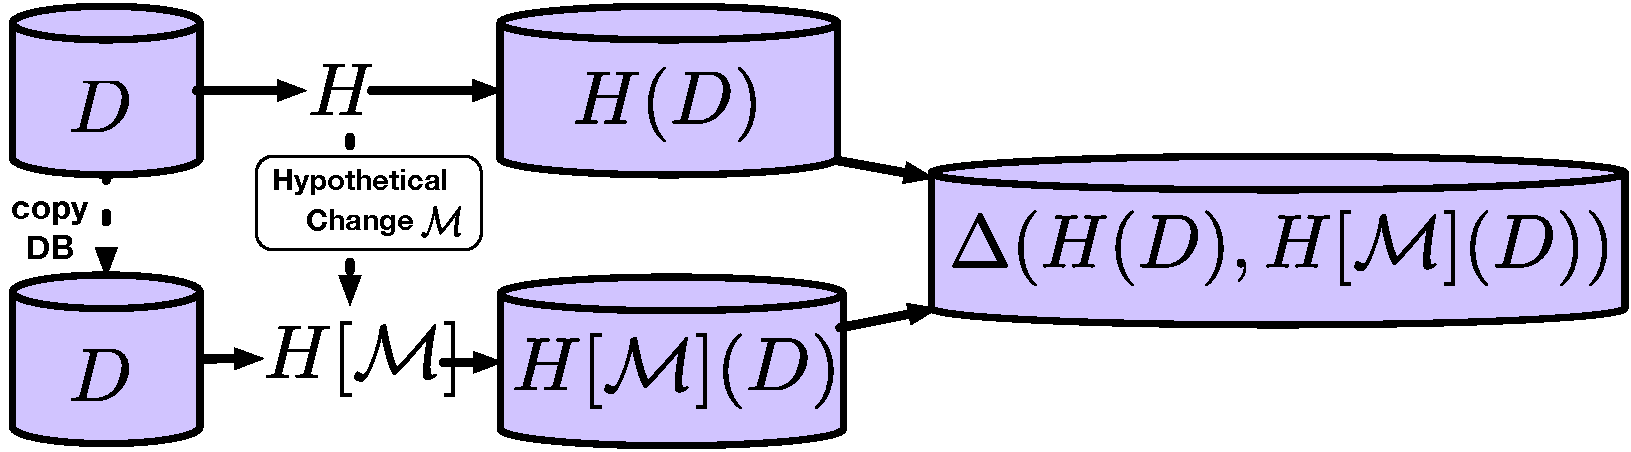
\includegraphics[width=0.9\linewidth]{brute-force-overview.pdf}
    \vspace{-4.5mm}
    \caption{The naïve method requires evaluating the modified history over a copy of the original database.}
    \label{fig:Naive-Method}
  \end{minipage}
  \begin{minipage}{1.0\linewidth}
    \centering
    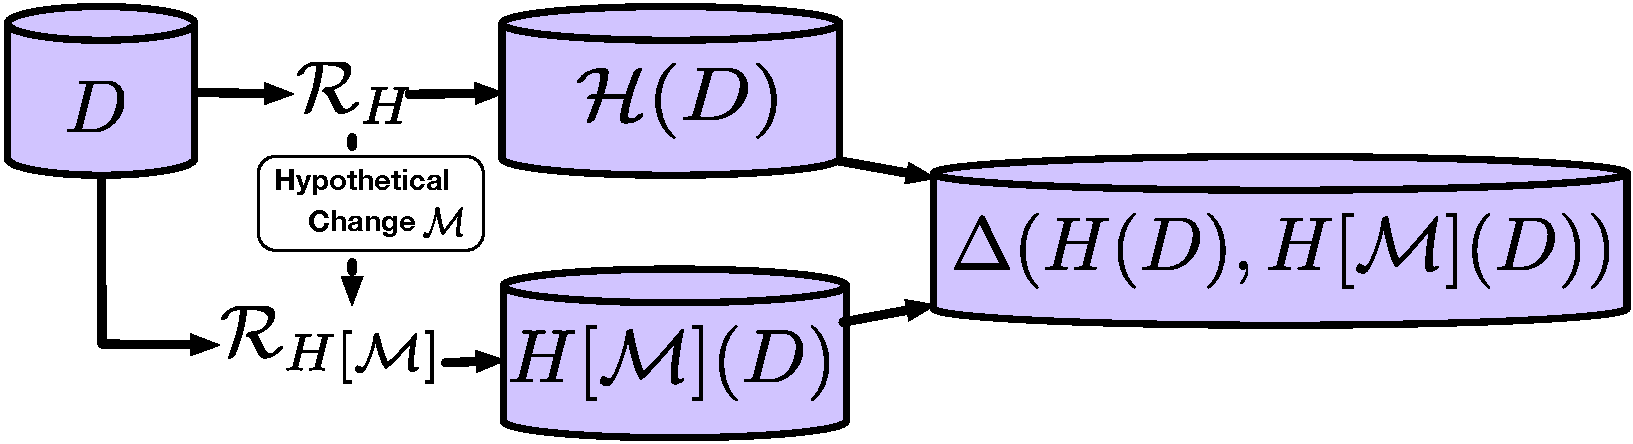
\includegraphics[width=0.9\linewidth]{reenact-overview.pdf}
    \vspace{-4.5mm}
    \caption{Reenactment-based method implemented in Mahif}
    \label{fig:Prop-Method}
  \end{minipage}
\end{figure}
%%%%%%%%%%%%%%%%%%%%%%%%%%%%%%%%%%%%%%%%

%%%%%%%%%%%%%%%%%%%%%%%%%%%%%%%%%%%%%%%%%%%%%%%%%%%%%%%%%%%%%%%%%%%%%%%%%%%%%%%%
A \textbf{naïve approach} for answering a \abbrHW is shown in \Cref{fig:Naive-Method}. This method creates a copy of the database as it was before the execution of the first update that has been modified by $\deltaHist$, and then executes the modified history on this copy. % It then executes the requested query on the copied database and the original. Finally, i
It then computes the symmetric difference between the current database state (which is the result of evaluating the original transactional history $\history$ over $\db$) and the database state that is the result of evaluating the modified history $\ahmod$ over the copy of database $\db$.  % is the answer to the historical what-if query. Note that
Note that this requires access to a past database state $\db$ before the execution of the first update of the history, e.g., we can use a DBMS with support for \textit{time travel} to access $\db$ (e.g., Oracle, SQLsever, DB2).
%
The naïve method requires additional storage to store the copy of $\db$ and the evaluation of the modified history results in a large amount of write I/O. % for updating data and write-ahead logging (WAL).
%
%
%
        %
However, an even larger concern is that the modifications  $\deltaHist$ may only affect a small fraction of the data and many updates in the history may be irrelevant for computing the symmetric difference. % That is, evaluating all updates of the modified history over all tuples in $\db$ is likely to be overkill.


%
%
%
        %

%%%%%%%%%%%%%%%%%%%%%%%%%%%%%%%%%%%%%%%%%%%%%%%%%%%%%%%%%%%%%%%%%%%%%%%%%%%%%%%%
Our \textbf{proposed method} is shown in \Cref{fig:Prop-Method}. In order to overcome the limitations of the naïve method, we propose Mahif as a system that answers \abbrHWs using reenactment~\cite{AG14,AG17,AG18}%  which is a declarative replay technique for transactional history by a temporal query.
% 
, a declarative technique for replaying transactional histories using queries.
% 
Our approach also uses time travel to access $\db$, the state of the database just before the time the first modified update was executed. In contrast to the naïve method, the database does not need to be copied. % Instead, time travel is used to get the state of the database before the update that is being modified, which is then the beginning state of the reenactment.
Instead, the modified history is reenacted over $\db$ by running a query $\ract{\ahmod}$.
Thus, reenactment has the advantage of not incurring write I/O.
The result of query $\ract{\ahmod}$ is equal to the result of executing $\ahmod$ over $\db$.  % to the naive method, we run the requested query on the result of the reenactment and original database state and then
We then compute the symmetric difference between the result of the modified history (returned by $\ract{\ahmod}$) and the current database state ($\history(\db)$) computed by reenacting $\history$ over $\db$. Reenacting $\history$, while seemingly redundant, allows us to develop novel optimizations which % dramatically decrease the amount data that needs to be processed and enables us to
exclude irrelevant updates from the history and irrelevant data from reenactment. % if they provably have no effect on the answer of the historical what-if query.
 %

% 

% 
%%%%%%%%%%%%%%%%%%%%%%%%%%%%%%%%%%%%%%%%%%%%%%%%%%%%%%%%%%%%%%%%%%%%%%%%%%%%%%%%
\partitle{Program Slicing}
To be able to identify updates that can safely be excluded from the evaluation of an \abbrHW, we introduce the notion of a \emph{slice}. A slice for a \abbrHW $\hwhatif$ is a subset of the updates from $\history$ and $\ahmod$ that is sufficient for computing the result of $\hwhatif$. We identify a property called tuple-independence which holds for a large class of updates (corresponding to SQL update and delete statements without joins and subqueries, and \lstinline!INSERT ... VALUES ...! statements). Tuple independence ensures that we can determine whether a subset of updates is a slice by testing for each individual tuple from the database whether the subset produces the same result for $\hwhatif$ than for the full histories. To improve the efficiency of slicing, we compress $\db$ into a set of constraints that compactly over-approximate the database. Inspired by program slicing and symbolic execution techniques~\cite{bucur14,luckow14}, and ideas from incomplete databases~\cite{AG85,IL84a}, we develop a technique that evaluates updates from a history over a single tuple symbolic instance (a tuple with variables as attribute values) subject to the constraints from the compressed database. The result of symbolic evaluation is a single tuple symbolic instance that encodes all possible tuples in the result of the history for any input tuple fulfilling the compressed database constraints. We then use a constraint solver % (MILP solver in our case)
  to determine whether a candidate slice produces the same result for $\hwhatif$ as the full histories for every possible input tuple. If that is the case, then it is safe to use the slice instead of $\history$ and $\ahmod$ to answer $\hwhatif$.
The cost of program slicing only depends on the number of updates in the history and the size of the constraints encoding the data distribution of the database. %Thus, % this method
% 
% 
% 


% 
% 
% 
% 
% 
% 
% 
% 

%%%%%%%%%%%%%%%%%%%%%%%%%%%%%%%%%%%%%%%%%%%%%%%%%%%%%%%%%%%%%%%%%%%%%%%%%%%%%%%%
\partitle{Data Slicing}
We also propose \emph{data slicing} to prune data that we can prove is irrelevant for computing the answer to a \abbrHW. Based on the observation that any tuple in the symmetric difference has to be affected by at least one statement that was modified by $\deltaHist$, we filter the input of reenactment to remove tuples which are guaranteed to not be affected by any update modified by $\deltaHist$. In addition to the class of queries supported by program slicing, data slicing is also applicable to insert statements with queries (\lstinline!INSERT ... SELECT! in SQL).
\BGDel{Our symbolic execution framework is of independent interest and can aide other static analysis task the require reasoning over multiple possible datasets or evaluation of updates over an incomplete database.}{Need space, maybe mention in future work}
%
%%%%%%%%%%%%%%%%%%%%%%%%%%%%%%%%%%%%%%%%
The main contributions of this paper are:
\begin{itemize}[noitemsep,topsep=0pt,parsep=0pt,partopsep=0pt,leftmargin=*]
%
%
%
\item
We formalize historical what-if queries and present a novel method for answering such queries based on reenactment.
%
%
%
%

%

\item We present two optimization techniques, \emph{program slicing} and \emph{data slicing}, which determine which updates and what data can be safely excluded when answering a \abbrHW.
  %

%

\item We demonstrate experimentally that our approach outperforms the naïve approach and that our optimizations result in significant additional performance improvements. % Note that the cost of program slicing is mostly determined by the number of updates in the history, but is independent of the database size. Thus, this method is suited well for larger database instances.

\end{itemize}

%%%%%%%%%%%%%%%%%%%%%%%%%%%%%%%%%%%%%%%%
%

%
%
%
%%%%%%%%%%%%%%%%%%%%%%%%%%%%%%%%%%%%%%%%%
%
%%%%%%%%%%%%%%%%%%%%%%%%%%%%%%%%%%%%%%%%
%
%
%
%%% Local Variables:
%%% mode: latex
%%% TeX-master: "historical_whatif"
%%% End:
